\section{Introduction}
Layered van der Waals solids are attractive thin-film materials because weak interlayer bonding enables exfoliation, heterostructure assembly, and growth on diverse substrates, while their electronic and transport properties remain sensitive to orientation and stacking.\cite{GeimGrigorieva2013,Jerng2013,Zhang2022Bi2Te3} Their structure is commonly measured with X-ray reflectivity, diffraction, and area-detector WAXS.\cite{Parratt1954,AlsNielsenMcMorrow2001,SmilgiesBlasini2007,Hexemer2015,Savikhin2020} Depending on the substrate and growth conditions, the layer normals may align with the film normal while the crystallites remain nearly random in in-plane azimuth.\cite{Zhang2022Bi2Te3} This uniaxially textured state is commonly called a two-dimensional (2D) powder: individual crystallites remain three-dimensional, but one crystallographic axis is preferentially aligned.\cite{Kaganer1999,Fischer2023MOFGIWAXS} At a single incidence angle, an area detector records Bragg peaks and diffuse intensity at the same time. These features provide complementary information about the film structure.\cite{SmilgiesBlasini2007,Hexemer2015,Savikhin2020}

Figure~\ref{fig:intro_2x3} illustrates this alignment and places the 2D-powder state between the single-crystal and 3D-powder limits in real, reciprocal, and detector space.

\begin{figure}[H]
  \centering
  \captionsetup{font=footnotesize}
  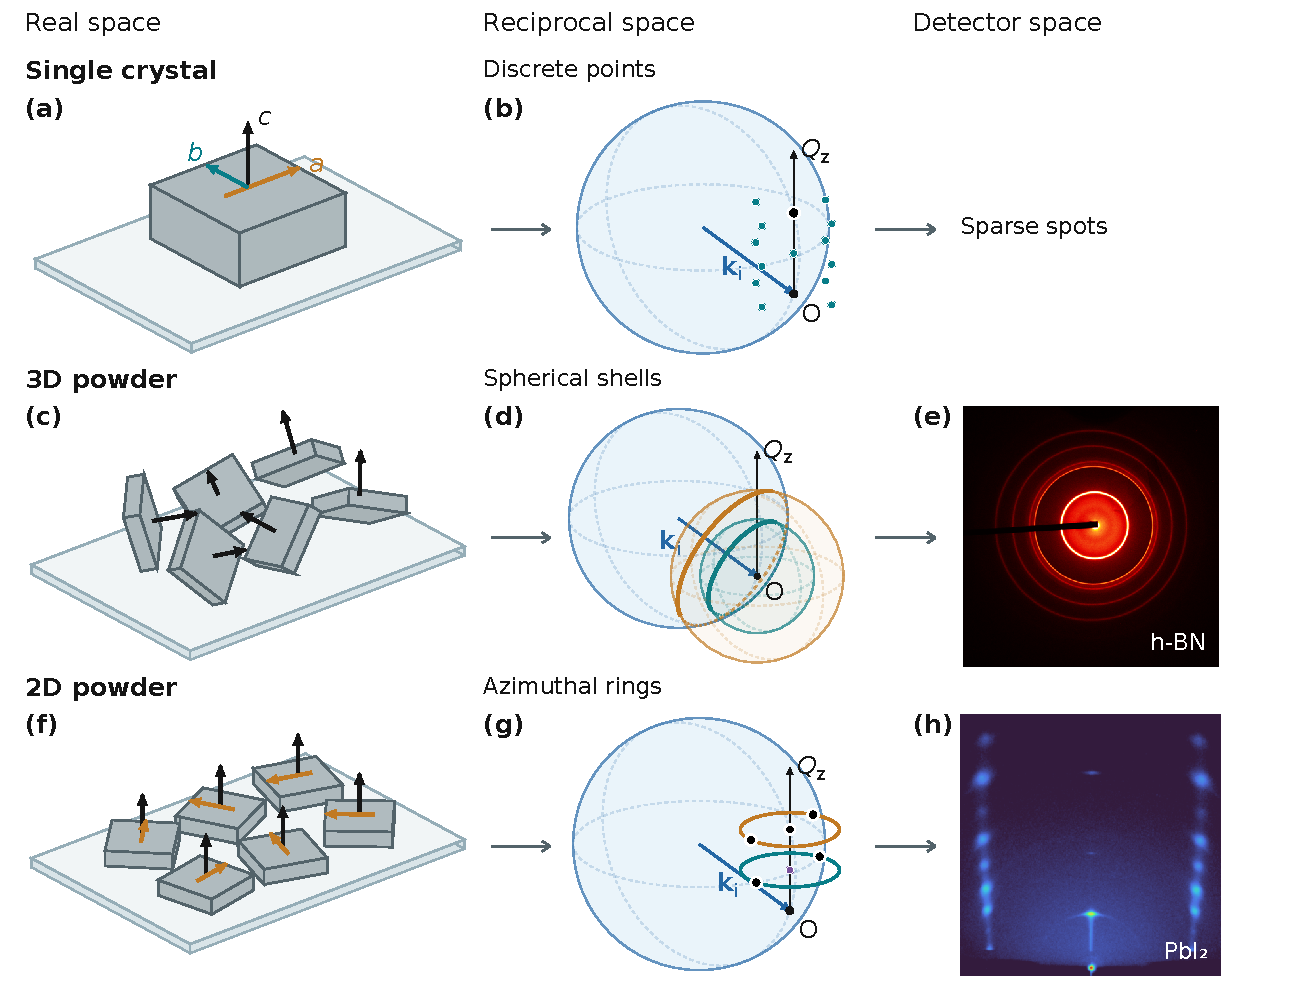
\includegraphics[width=\linewidth]{figures/intro/orientational_limits_reference_journal.pdf}
  \caption[Diffraction across three orientational limits]{Crystallite orientation controls the reciprocal-space distribution and resulting detector pattern. A single crystal gives discrete reciprocal-lattice points (a,b). Random three-dimensional orientations give spherical shells (c,d) and Debye--Scherrer rings, illustrated by h-BN (e). A common film normal with random in-plane azimuth gives off-axis reciprocal-space rings (f,g), whose Ewald intersections produce paired off-specular features, illustrated by PbI$_2$ (h). Arrows between columns indicate this correspondence. Black real-space arrows mark crystallite normals, orange arrows mark an in-plane direction, and $a,b,c$ label crystal axes. Blue spheres show the Ewald construction, with incident wavevector $\mathbf{k}_i$, reciprocal origin $O$, and film-normal axis $Q_z$. Teal and orange distinguish reflection loci. Black points and thick colored curves mark selected intersections, dashed curves are construction guides, and the purple axial point is unselected.}
  \label{fig:intro_2x3}
\end{figure}

Here $\mathbf{k}_i$ and $\mathbf{k}_f$ are the incident and exit wavevectors, and $\mathbf Q=\mathbf{k}_f-\mathbf{k}_i$ is the momentum transfer. The Ewald sphere is centered at $-\mathbf{k}_i$, passes through the reciprocal-space origin, and has radius $|\mathbf{k}_i|=2\pi/\lambda$. Elastic diffraction selects reciprocal-space intensity satisfying $|\mathbf{k}_i+\mathbf Q|=|\mathbf{k}_i|$, and each selected $\mathbf Q$ defines $\mathbf{k}_f=\mathbf{k}_i+\mathbf Q$.\cite{AlsNielsenMcMorrow2001} A single crystal supplies isolated reciprocal-lattice points, while random 3D orientations spread each reflection over a spherical shell. In a 2D powder, random in-plane azimuth spreads each off-axis reflection into a ring about the film-normal reciprocal-space axis, while $(00L)$ intensity remains near that axis.\cite{Kaganer1999,SmilgiesBlasini2007} The Ewald sphere generally intersects an off-axis ring at two points, which map to paired detector features.\cite{SmilgiesBlasini2007,Hexemer2015,Smilgies2005Rods} Mosaicity and other experimental effects broaden these ideal intersections into arcs and cap-like intensity while preserving the same elastic condition.

Figure~\ref{fig:area_detector_overview} shows a representative measured PbI$_2$ pattern.

\begin{figure}[H]
  \centering
  \captionsetup{font=footnotesize}
  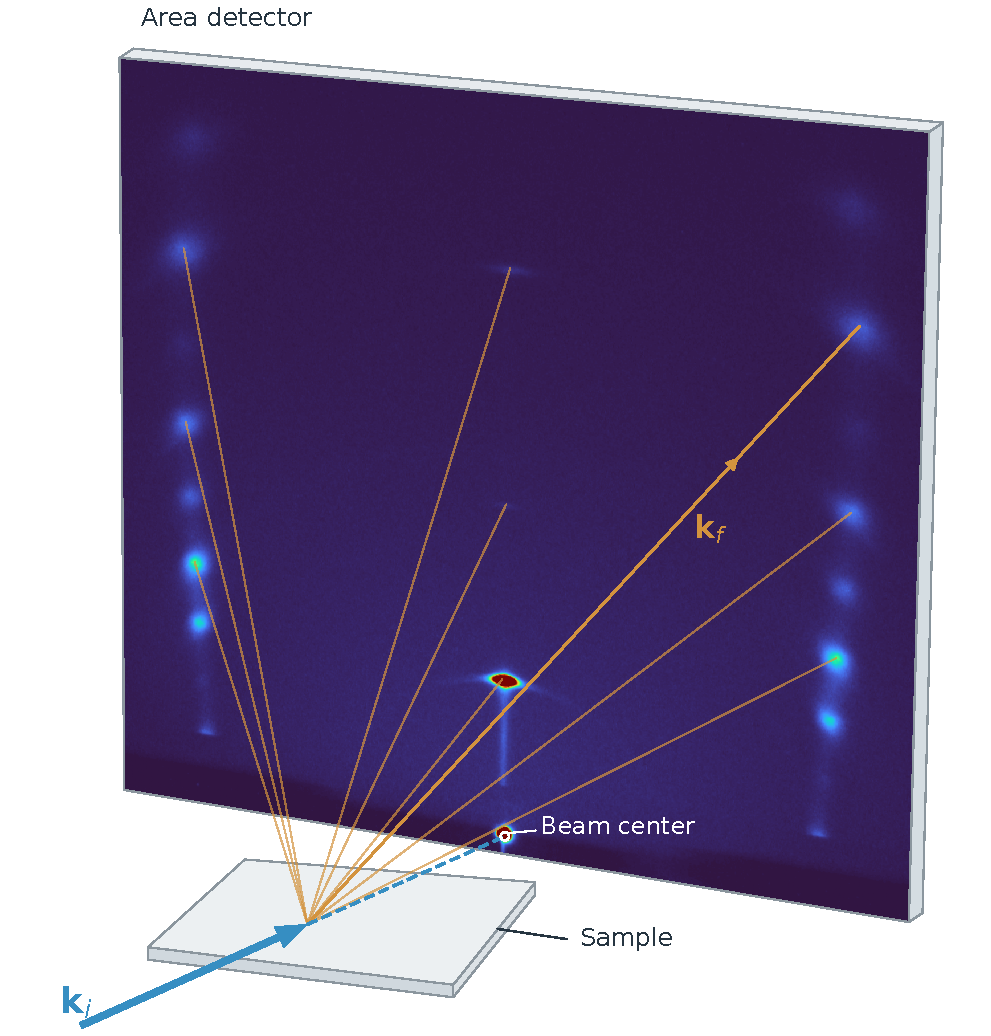
\includegraphics[width=0.62\linewidth]{figures/intro/area_detector_overview_journal.pdf}
  \caption[Area-detector measurement of a 2D powder]{An area detector records multiple diffraction features simultaneously, at positions displaced from the undeflected-beam reference. The displayed pattern is measured from a PbI$_2$ film. The blue arrow marks the incident wavevector $\mathbf{k}_i$, and its dashed continuation reaches the beam center, marked by an open circle. Orange rays connect the sample to selected diffraction features, with one scattered wavevector $\mathbf{k}_f$ identified by an arrowhead. Peaks, arcs, and intensity between peaks are recorded in the same exposure.}
  \label{fig:area_detector_overview}
\end{figure}

Standard WAXS workflows often integrate area-detector images into one-dimensional profiles, an effective representation for nearly isotropic powders.\cite{Ashiotis2015,Hexemer2015,Savikhin2020,Reus2024} For a 2D powder, retaining the radial and transverse detector directions keeps the specular and off-specular features as separate, complementary constraints. Stacking disorder is also commonly treated with one-dimensional interference models.\cite{HendricksTeller1942,Treacy1991,CasasCabanas2016} Full orientation-distribution-function refinements can represent arbitrary textures,\cite{WenkVanHoutte2004,Lutterotti2004TSF,VonDreele1997,LutterottiVasinWenk2014} while more constrained cases can be represented by lower-dimensional preferred-orientation kernels\cite{March1932,Dollase1986} or a small number of epitaxial variants.\cite{Smilgies2000POPOP} The present work considers the 2D-powder limit. The approximately azimuthally symmetric measured features motivate axial symmetry about the film normal and a compact out-of-plane mosaicity distribution. We therefore use the off-specular arcs and axial-family profiles as complementary constraints on the same orientation model.

The optical boundary conditions follow established grazing-incidence formalisms,\cite{Sinha1988,Renaud2009,Hexemer2015,Savikhin2020} while the reciprocal-rod geometry and allowed-reflection locations build on reciprocal-space mapping and detector-space indexing for oriented films.\cite{SmilgiesBlasini2007,Smilgies2005Rods,Breiby2008,SmilgiesLi2026IndexGIXS} For these data, wavelength bandwidth, beam divergence, refraction, sample misalignment, mosaicity, and stacking disorder can redistribute intensity in overlapping ways. We therefore evaluate them within one calculation.
Source position and divergence are sampled from the measured Gaussian beam distributions, while wavelength is sampled from the input wavelength spectrum. For each $\mathbf{k}_i$, the model constructs a structure function, applies the corresponding Ewald condition, and maps the accepted intensity to the calibrated detector. The forward calculation incorporates these corrections. Applying identical integration regions to the measured and calculated detector intensities preserves the radial and transverse information.

Figures~\ref{fig:ordered_bi2se3_test} and~\ref{fig:ordered_bi2te3_test} present the Bi$_2$Se$_3$ and Bi$_2$Te$_3$ detector comparisons and selected profiles at nominal $5^\circ$ incidence, a condition included in the refinement. The panels separate the off-axis rod families from the axial response. These ordered-film test cases are followed by the staged refinement workflow and then the PbI$_2$ stacking-disorder extension.
